\subsection{Combinations of Continuous Functions}

\ex{1}
\begin{enumerate}[label=(\alph*)]
    \item 
    \begin{proof}
        For $\varepsilon>0$ choose
        $\delta = \varepsilon^3$ then $|\sqrt[3]{x}| < \varepsilon$
        for $|x| < \delta$.
    \end{proof}

     \item 
    \begin{proof}
        For $\varepsilon>0$ choose $\delta=\varepsilon\sqrt[3]{c^2}$
        then
        \begin{align*}
            |\sqrt[3]{x} - \sqrt[3]{c}| &= \frac{|x-c|}{|\sqrt[3]{x^2} + \sqrt[3]{xx} +\sqrt[3]{c^2}|} \\
            &\leq \frac{|x-c|}{\sqrt[3]{c^2}} \\
            &< \varepsilon
        \end{align*}
    \end{proof}
\end{enumerate}

\ex{2}
\begin{enumerate}[label=(\alph*)]
    \item 
    \begin{proof}
        Becuase $g$ is continuous then choose $\delta_1$ s.t. 
        \begin{align*}
            |g(x)-g(c)|<\varepsilon
        \end{align*}
        which requires $|f(x)-f(c)|<\delta_1$ for some $\delta_1>0$.
        However, since $f(x)$ is continuous this will occur for $|x-c|<\delta$
        for some $\delta>0$.
    \end{proof}

    \item
    \begin{proof}
        For any sequence $(x_n)\rightarrow c$ $f(x_n)\rightarrow f(c)$.
        However, $g$ is also continuous so $g(y_n)\rightarrow g(y)$
        for any sequence so in particular choose sequence $f(x_n)$. Then 
        $g(f(x_n))\rightarrow g(f(x))$
        
        So for any seqeunce $(x_n)\rightarrow c$ $(g\circ f)(x_n) \rightarrow (g\circ f)(x)$
        so $g\circ f$ is continuous.
    \end{proof}
\end{enumerate}

\ex{3}
\begin{proof}
    For $\varepsilon>0$ choose $\delta=\varepsilon/a$ then  
    \begin{align*}
        |ax+b - ac - b| = a|x-c| < \varepsilon
    \end{align*}
\end{proof}


\ex{4}
\begin{enumerate}[label=(\alph*)]
    \item 
    \begin{proof}
        If point in $\mathbb{Z}$ then choose $\delta = 1$, then 
        $|x-c| < \delta \Rightarrow x=c$ so $|f(x)-f(c)|=0 < \varepsilon$.
    \end{proof}

    \item
    \begin{proof}
        For 
        isolated points the defintiion of continuity is automatically 
        satisfied since there exists $V_\delta(x)\cap A=\{x\}$ 
        for every $x\in A$.
        For such a $\delta$ $|f(x)-f(c)| = 0$ since $|x-c|=0$ which is allowed 
        in the definition of continuity.
    \end{proof}
\end{enumerate}

\ex{5}
This statement cannot be true for isolated points so we 
assume $c$ is a limit point.
\begin{proof}
    Since $g$ is continuous then 
    \begin{align*}
        |g(x)-g(c)| < |g(c)|
    \end{align*}
    for $|x-c|<\delta$ for some $\delta>0$. This implies $g(x)\neq 0$ given 
    $|x-c|<\delta$. Hence $\frac{f(x)}{g(x)}$ is well-defined
    given $|x-c|<\delta$.
\end{proof}

\ex{6}
\begin{enumerate}[label=(\alph*)]
    \item 
    \begin{proof}
        For any $c\in \mathbb{R}$ we can define a rational sequence s.t. 
        $(q_n)\rightarrow c$ and irrational sequence s.t. $(i_n)\rightarrow c$.
        Hence $g(q_n)\rightarrow 1$ but $g(i_n)\rightarrow 0$. Hence, 
        $g$ fails by the sequential criterion for continuity.
    \end{proof}

    \item 
    \begin{proof}
        For some $q=\frac{m}{n} \in \mathbb{Q}$ choose 
        $0<\varepsilon<1/n$, then for any $\delta>0$, 
        $|x-q|<\delta$ will contain irrational value $y$ 
        so $|t(y)-t(q)|=1/n\geq \varepsilon$ so $t$ is not 
        continuous at $q$.
    \end{proof}

    \item 
    TBC
\end{enumerate}

\ex{7}
\begin{proof}
    Consider $x\in K^c$, in \Ex{5} we showed that for continuous functions there
    exists some open interval where the function is non-zero around $h(x)$.
    Hence for every $x\in K^c$ there exists an open interval in $K^c$ so 
    $K^c$ is open which implies $K$ is closed.
\end{proof}

\ex{8}
\begin{enumerate}[label=(\alph*)]
    \item 
    \begin{proof}
        Take some irrational point $c\in \mathbb{I}$, then because $\mathbb{Q}$
        is dense in $\mathbb{R}$ then there exists sequence $(q_n)\rightarrow c$
        where $(q_n) \in \mathbb{Q}$. Hence,
        \begin{align*}
            0 = \lim f(q_n) = f(c)
        \end{align*}
    \end{proof}

    \item 
    \begin{proof}
        Define $h = f-g$ which is continuous on $\mathbb{R}$. 

        Take some irrational point $c\in \mathbb{I}$, then because $\mathbb{Q}$
        is dense in $\mathbb{R}$ then there exists sequence $(q_n)\rightarrow c$
        where $(q_n) \in \mathbb{Q}$. Hence,
        \begin{align*}
            0 = \lim h(q_n) = h(c)
        \end{align*}
        which implies $h(c)=0$ for all $c\in \mathbb{R}$ so $f(c)=g(c)$ for all 
        $c\in \mathbb{R}$.
    \end{proof}
\end{enumerate}

\ex{9}
\begin{enumerate}[label=(\alph*)]
    \item 
    \begin{proof}
        For some $\varepsilon>0$ choose $\delta = \varepsilon/c$ and 
        fix $y$, then  
        \begin{align*}
            |f(x)-f(y)| \leq c|x-y| < \varepsilon
        \end{align*}
        so $f$ is continous at $y$. Since $y$ was arbitrary then $f$ is
        continous on $\mathbb{R}$.
    \end{proof}

    \item
    \begin{proof}
        Now observe 
        \begin{align*}
            |y_{m+1}| &= |f(y_m)-f(y_{m-1})| \\ 
            &\leq c |y_m - y_{m-1}| \\
            \Rightarrow |y_n - y_m| &\leq c^l|y_{n-l} - y_{m-l}| \\
            \Rightarrow |y_n - y_m| &\leq c^{m-1}|y_{n-(m-1)} - y_{l}| \\
            \Rightarrow |y_{m+1} - y_m| &\leq c^{m-1}|y_2 - y_{l}|
        \end{align*}

        Let $n=m+s$ with $s>0$ so that $n>m$, then 
        \begin{multline*}
            |y_{m+s} - y_m| = |y_{m+s} - y_{m+s-1} \\ + y_{m+s-1} - \cdots + y_{m+1} - y_m| \\
            \leq |y_{m+s} - y_{m+s-1}| + |y_{m+s-1} - y_{m+s-2}| \\  + \cdots + |y_{m+1} - y_m| \\
            \leq (c^{m+s-2}+c^{m+s-2}+\cdots+c^{m-1})|y_2-y_1| \\
            = \sum_{l=m-1}^{m+s-2} c^l |y_2-y_1| 
            = \frac{c^{m-1}(c^s-1)}{c-1} |y_2-y_1|
        \end{multline*}

        Now we require that
        \begin{align*}
            \frac{c^{m-1}(c^s-1)}{c-1} |y_2-y_1| < \varepsilon
        \end{align*}
        for any $\varepsilon>0$.

        Now $c-1 = -|c-1|$ and $c^s-1 = -|c^s-1|$ since $s\geq 1$ and $c<1$. So
        \begin{align*}
            \frac{c^{m-1}(c^s-1)}{c-1} |y_2-y_1| &= \frac{c^{m-1}|c^s-1|}{|c-1|} |y_2-y_1|
        \end{align*}
        Rearranging this expression we get
        \begin{align*}
            m > \log_c\left( \frac{|c-1|\varepsilon}{|c^s-1||y_2-y_1|} \right) + 1
        \end{align*}
        so for $n>m\geq N>\log_c\left( \frac{|c-1|\varepsilon}{|c^s-1||y_2-y_1|} \right) + 1$
        \begin{align*}
            |y_n-y_m| <\varepsilon
        \end{align*}
    \end{proof}

    \item
    \begin{proof}
        Observe,
        \begin{align*}
            f(y) = \lim f(y_n) = \lim y_{n+1} = y
        \end{align*}
        Hence $y$ is a fixed point. Suppose $x$ is also a fixed point then 
        \begin{align*}
            |x-y| = |f(x)-f(y)| \leq c|x-y|
        \end{align*}
        However, $|x-y| \leq c |x-y|$ is only true if $|x-y|=0$ since $0<c<1$.
        So $y$ is a unique fixed point.
    \end{proof}

    \item
    \begin{proof}
        We have shown that choosing any $x\in \mathbb{R}$ then 
        we can define sequence $x_{n+1}=f(x_n)$ i.e. $(x, f(x), f(f(x)), ...)$
        We know from (b) that $(x_n)\rightarrow x$ and defines a fixed point 
        of $f$. Since the fixed point of $f$ is unique and 
        we know $y$ is a fixed point then if $x$ is
        also a fixed point then $x=y$.
    \end{proof}
\end{enumerate}

\ex{10}
\begin{enumerate}[label=(\alph*)]
    \item 
    \begin{proof}
        $f(0) = f(0)+f(0) \Rightarrow f(0)=0$.
    \end{proof}

    \begin{proof}
        $0=f(0)=f(x-x)=f(x)+f(-x) \Rightarrow f(-x)=f(x)$.
    \end{proof}

    \item
    Suppose $f$ is continuous at $x=0$ then 
    \begin{align*}
        |f(x)|< \varepsilon
    \end{align*}
    for $|x|<\delta$. Then for $c\in \mathbb{R}$
    \begin{align*}
        |f(x)-f(c)| = |f(x-c)|
    \end{align*}
    However, $|f(x-c)|<\varepsilon$ given $|x-c|<\delta$.

    \item
    \begin{proof}
        $f(n) = f(1+1+\cdots+1) = f(1)+f(1)+\cdots+f(1) = kn$.
    \end{proof}

    \begin{proof}
        $f(z) = f(\text{sgn}(z)|z|) = \text{sgn}(z)f(|z|) = \text{sgn}(z)k|z| = kz$.
    \end{proof}

    \begin{proof}
        Let $r=m/n$, then $nf(m/n)=f(m)=km \Rightarrow f(m/n)=km/n$.
    \end{proof}

    \item
    \begin{proof}
        For any $(q_n)\in \mathbb{Q}$ s.t. $(q_n) \rightarrow c \in \mathbb{R}$ then 
        since $f$ is continuous then 
        \begin{align*}
            f(c) = \lim f(kq_n) = k \lim f(q_n) = kc
        \end{align*}
        Hence, $f(c)=kc$ for any $c\in \mathbb{R}$.
    \end{proof}
\end{enumerate}

\ex{11}
\begin{enumerate}[label=(\alph*)]
    \item 
    \begin{align*}
        g(x) = \begin{cases}
            1 & x\in \mathbb{Z} \\ 
            0 & \text{otherwise}
        \end{cases}
    \end{align*}

    \begin{figure}[h]
        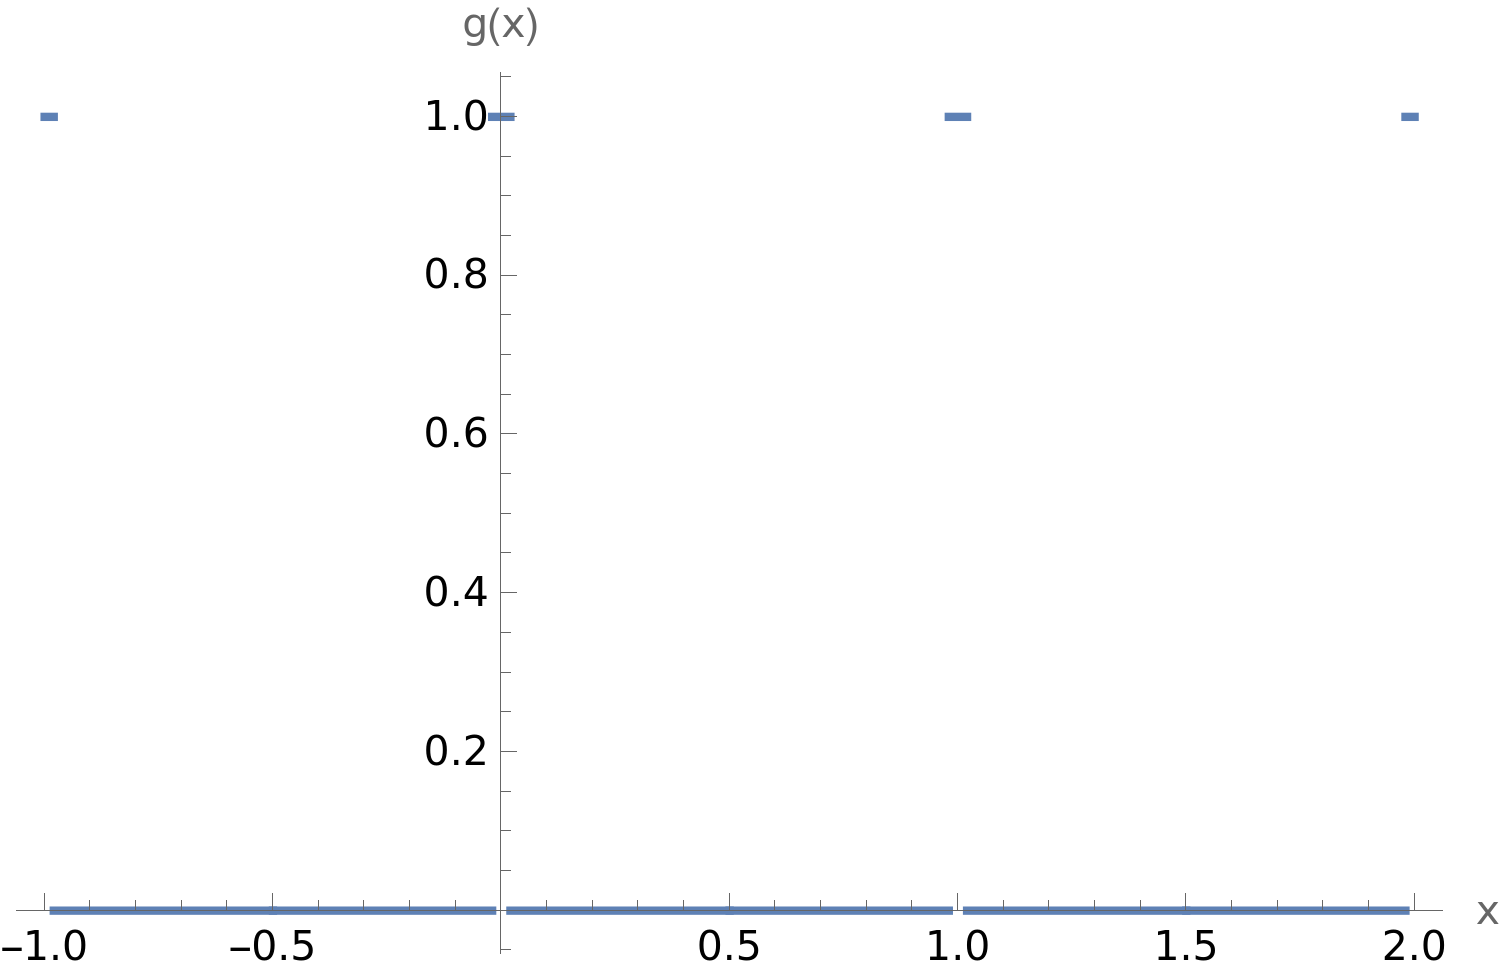
\includegraphics[width=0.4\textwidth]{4 Functional Limits and Continuity/4_3_11/4_3_11_a.png}
        \caption[]{\Ex{11} (a)}
        \label{fig:4_3_11_a}
    \end{figure}

    \item
    \begin{align*}
        g(x) = \begin{cases}
            x & x \in \mathbb{Q} \text{ and } 0<x<1 \\ 
            x^2 & x \in \mathbb{I} \text{ and } 0<x<1 \\ 
            0 & x \leq 0 \\
            1 & x \geq  1
        \end{cases}
    \end{align*}

    \begin{figure}[h]
        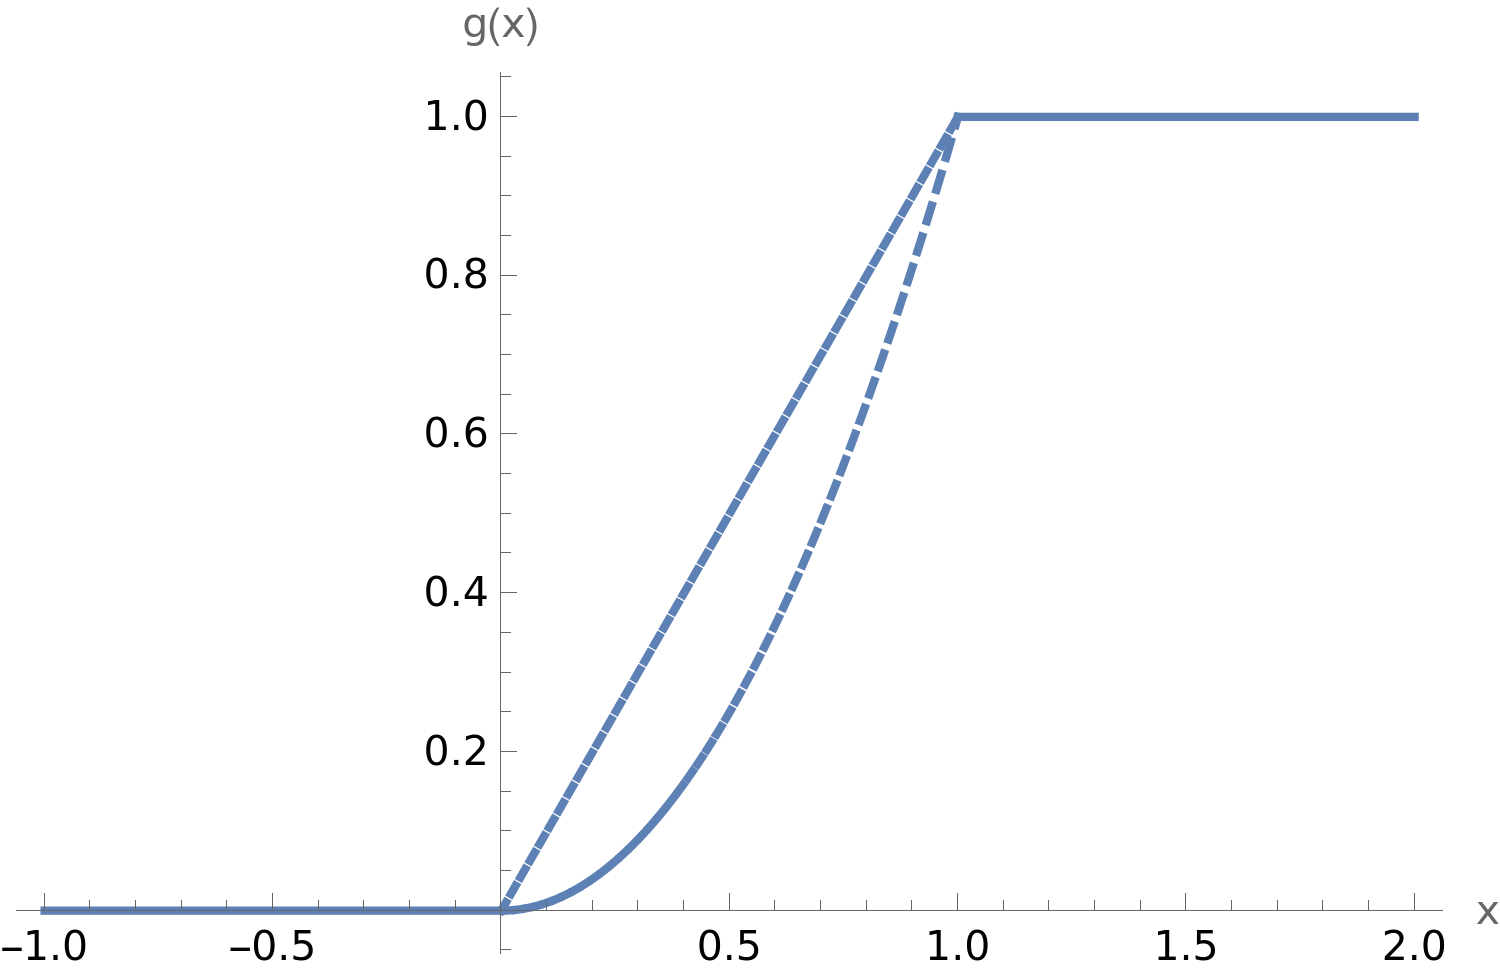
\includegraphics[width=0.4\textwidth]{4 Functional Limits and Continuity/4_3_11/4_3_11_b.png}
        \caption[]{\Ex{11} (b)}
        \label{fig:4_3_11_b}
    \end{figure}

    \item
    \begin{align*}
        g(x) = \begin{cases}
            1 & x \in \mathbb{Q} \text{ and } 0<x<1 \\ 
            0 & x \in \mathbb{I} \text{ and } 0<x<1 \\ 
            0 & x\leq 0 \text{ or } x\geq 1
        \end{cases}
    \end{align*}

    \begin{figure}[h]
        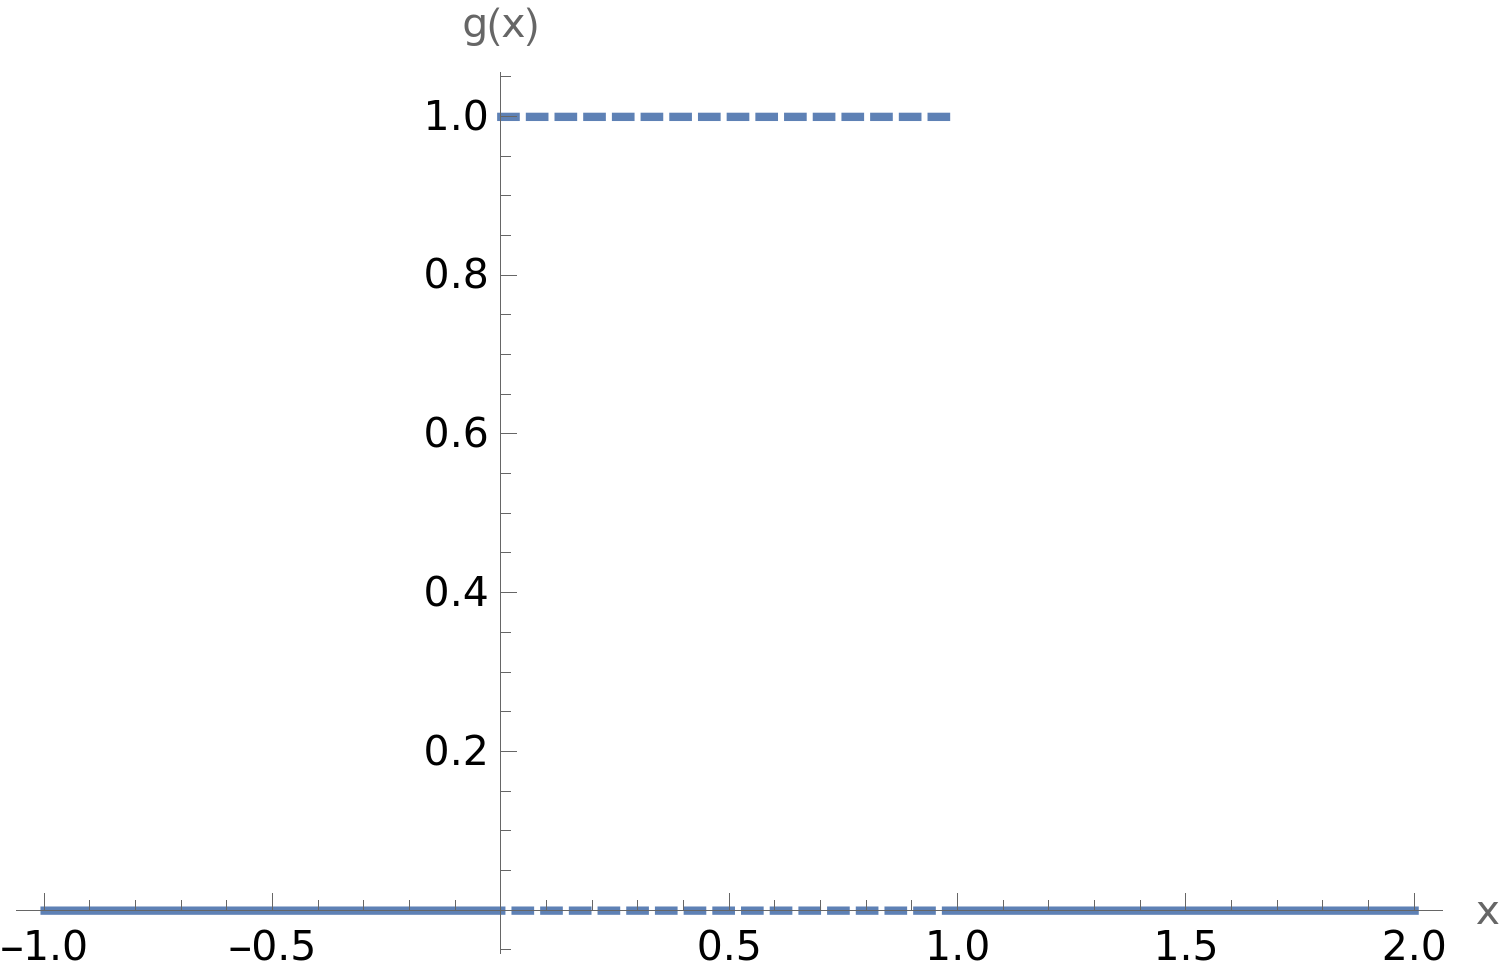
\includegraphics[width=0.4\textwidth]{4 Functional Limits and Continuity/4_3_11/4_3_11_c.png}
        \caption[]{\Ex{11} (c)}
        \label{fig:4_3_11_c}
    \end{figure}

    \item
    \begin{align*}
        g(x) = \begin{cases}
            x & x=1/n \text{ for some } n\in \mathbb{N} \\ 
            0 & \text{ otherwise } 
        \end{cases}
    \end{align*}

    \begin{figure}[h]
        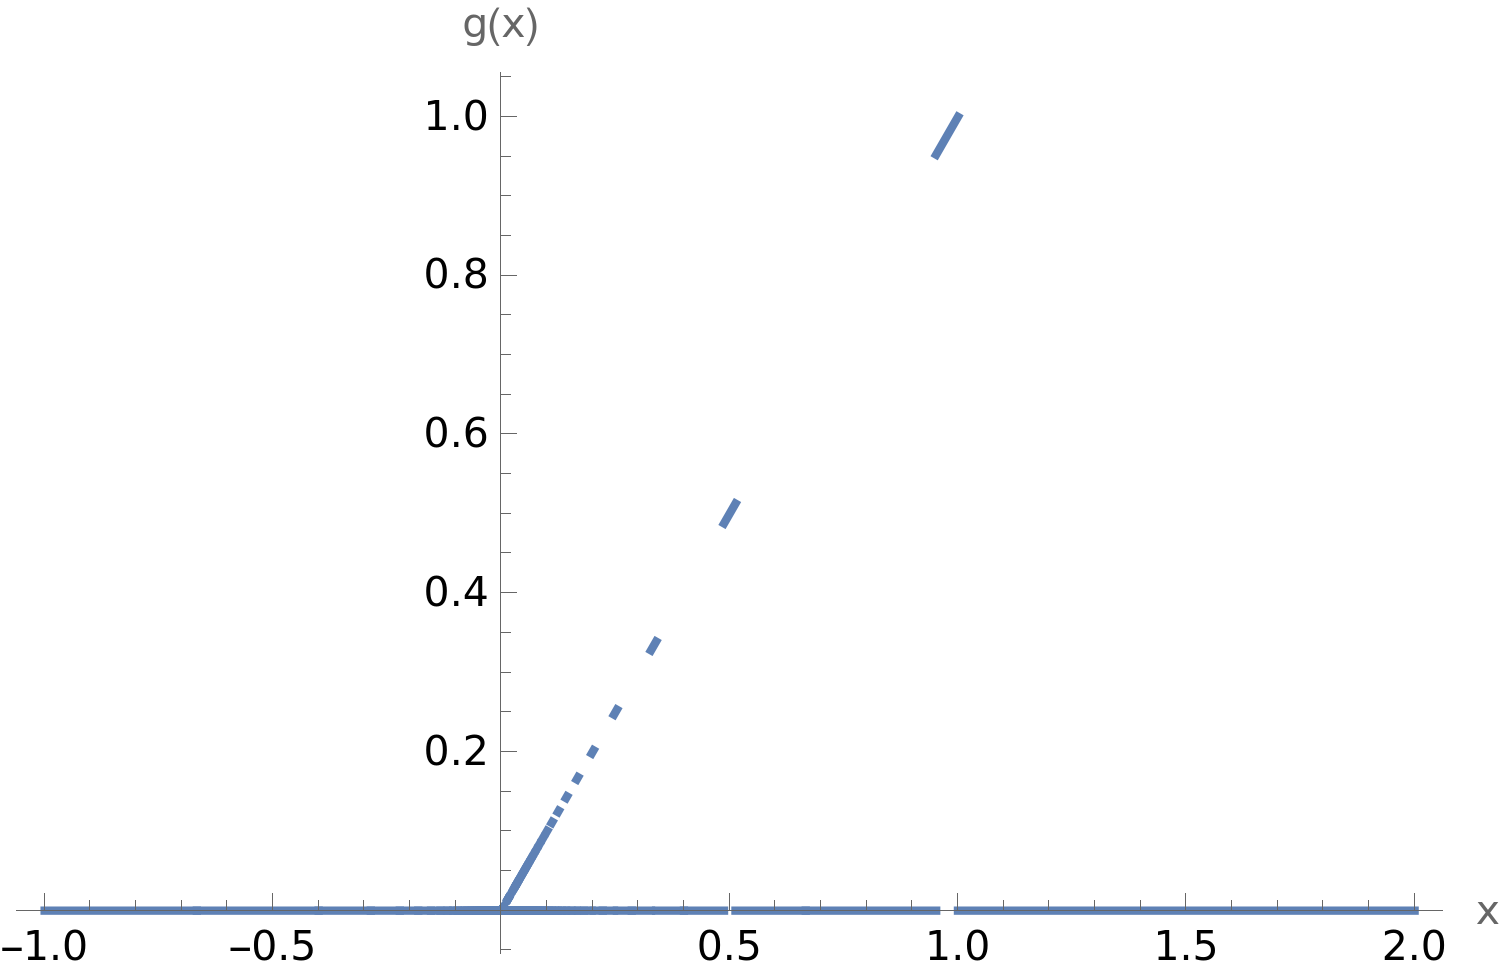
\includegraphics[width=0.4\textwidth]{4 Functional Limits and Continuity/4_3_11/4_3_11_d.png}
        \caption[]{\Ex{11} (d)}
        \label{fig:4_3_11_d}
    \end{figure}
\end{enumerate}


\ex{12}
\begin{enumerate}[label=(\alph*)]
    \item 
    \begin{proof}
        For some $c\in C$ and any $\delta>0$ we know $c\in C_n$ for all $n$.
        How the size of each interval in $C_n$ is $1/3^n$ so we choose $n$ such 
        that each interval is less that $\frac{1}{3^n 2} < \delta$ i.e. 
        $\delta$ is twice as large as interval. Lets call this interval $I$.
        Now $c\in I$ and since $|I|< \delta /2 $ then there exist points $x\in C_n$ 
        s.t. $|x-c|<\delta$ but $x\not\in C_n$ so we know 
        that $|g(x)-g(c)|=1$. Hence, $g$ will always fail to be continuous since
        we can always choose $0<\varepsilon < 1$.
    \end{proof}

    \item 
    \begin{proof}
        If $c\not\in C$ then there exists $n$ s.t. $c\in C_n$ but
        $c\not\in C_{n+1}$. Since $C_{n+1}$ has the interval of 
        length $\frac{1}{3^{n+1}}$ with $c$ in the removed region then 
        there exists an open neighbourhood around $c$ not in $C_{n+1}$.
        Lets call this $V_\delta(c)$, then for any $\varepsilon>0$ 
        $g(x)\in V_\varepsilon(0)$ given $x\in V_\delta(c)$.
    \end{proof}
\end{enumerate}